\chapter{El semicilindro}
\label{semicilindro-1}

\section{Diferencias}

\lettrine[ante=\raisebox{-1.5ex}{\LARGE ---¿},lines=2]{T}{e acordás
  del} reloj de Sol digital..? ---preguntó al día siguiente Antonia,
con aire inocente.

---Claro ---Cecilia respondió con una sonrisa burlona---; pensé que
nunca lo íbamos a empezar.

---Su cuerpo principal es un semicilindro; en él haremos luego los
orificios que le den sentido y lo justifiquen. Así que te sugiero
comenzar definiendo un nuevo objeto: el `semicilindro' ---propuso
Antonia, y Cecilia, con tal de avanzar, asintió.

---En principio ---continuó Antonia---, se me ocurre que un
semicilindro debe quedar caracterizado por su altura y su radio; para
no desentonar con el resto del lenguaje, y tomando en cuenta el
estrecho parentezco entre un semicilindro y un `\lstinline!cylinder!',
llamémoslos \texttt{h} y \texttt{r}:\footnote{Esta decisión de Antonia
  debió haberse inspirado en el denominado ``Principio de la mínima
  perplejidad'' (\emph{Principle of Least Astonishment}), que forma
  parte de la cultura informática desde la década de 1970, por lo
  menos. (Nota del Editor)}

  % \begin{center}
  % \begin{minipage}[]{.6\textwidth}
    \begin{lstlisting}
module semicilindro(h,r){
}
    \end{lstlisting}
  % \end{minipage}\hfill
  % \begin{minipage}[]{.4\textwidth}
  %     \centering
  %     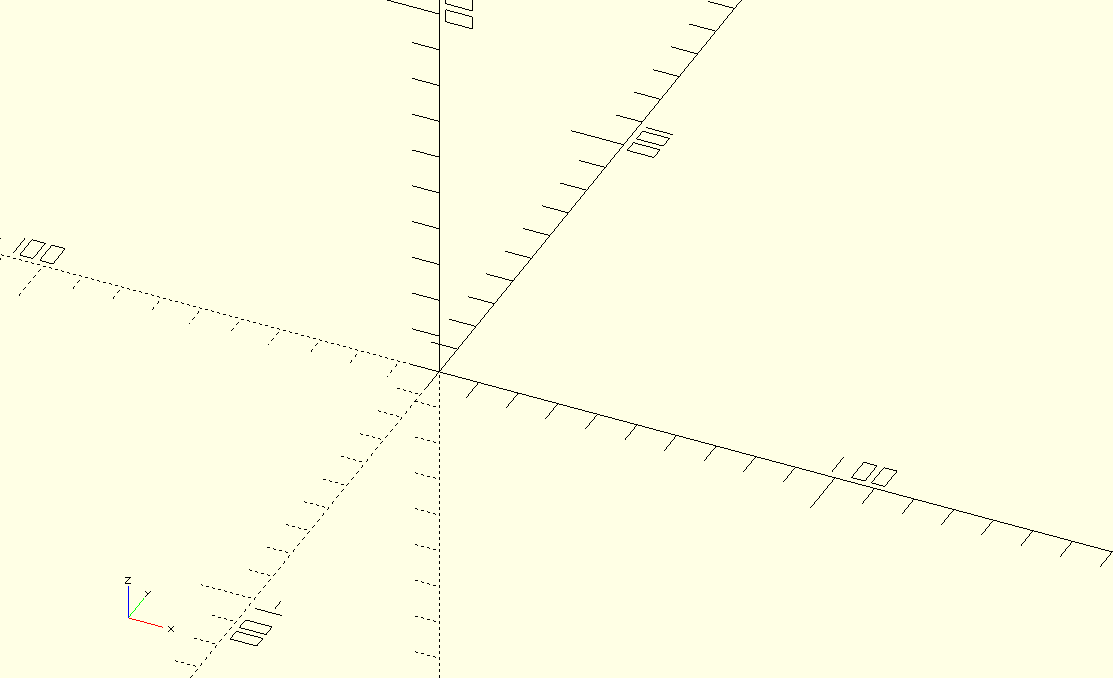
\includegraphics[width=.6\textwidth]{imagenes/vacio}
  %   \end{minipage}
  % \end{center}


    ---Ahora bien ---prosiguió Antonia---; podemos contemplar un
    semicilindro como un cilindro al que le cercenaron una mitad; por
    supuesto, esa operación elemental de `corte' no podía faltar entre
    las posibilidades de \openscad{}. Se logra con la operación
    \lstinline!difference()!. Dejame mostrate antes un ejemplo suelto:

%  \begin{center}
%  \begin{minipage}[]{1\textwidth}
    \begin{lstlisting}
$fn=100;
      
translate([-100,0,0])
  cube([30,30,30],center=true);  

translate([-50,0,0])
  cylinder(h=60,r=5,center=true);  

difference() {
  cube([30,30,30],center=true);
  cylinder(h=60,r=5,center=true);
}
    \end{lstlisting}%$
  % \end{minipage}\hfill
  % \end{center}  

    \begin{figure}[ht]
      \centering
      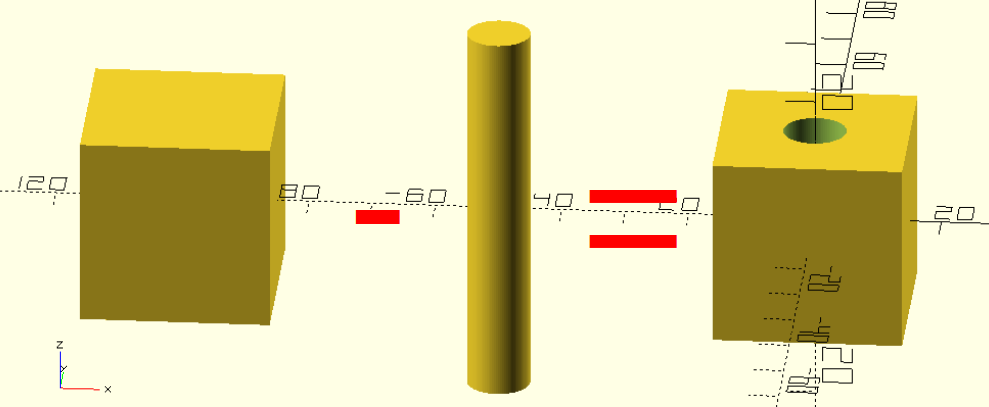
\includegraphics[width=.75\textwidth]{imagenes/diferencia-signos}      
      \caption{Antonia ofrece un ejemplo de la operación
        \lstinline!difference()!.}
      \label{fig:diferencia-signos}
    \end{figure}

  
    \guillemotright Las líneas 3 a 7 fueron para hacerme la canchera:
    sólo sirven para mostrar los elementos que luego resto
    efectivamente en las líneas 9 a 12. La idea es que
    \lstinline!difference()! encierra entre llaves dos o más
    elementos, `restando' del primero cada uno de los siguientes. A
    ver qué te parece este otro ejemplo:

  % \begin{center}
  % \begin{minipage}[]{1\textwidth}
    \begin{lstlisting}
$fn=100;
difference() {
  cube([30,30,30],center=true);
  cylinder(h=60,r=5,center=true);
  rotate([90,0,0])
   cylinder(h=60,r=5,center=true);
  rotate([0,90,0])
   cylinder(h=60,r=5,center=true);
}
    \end{lstlisting}%$
  % \end{minipage}\hfill
% \end{center}


    \begin{figure}[ht]
      \centering
      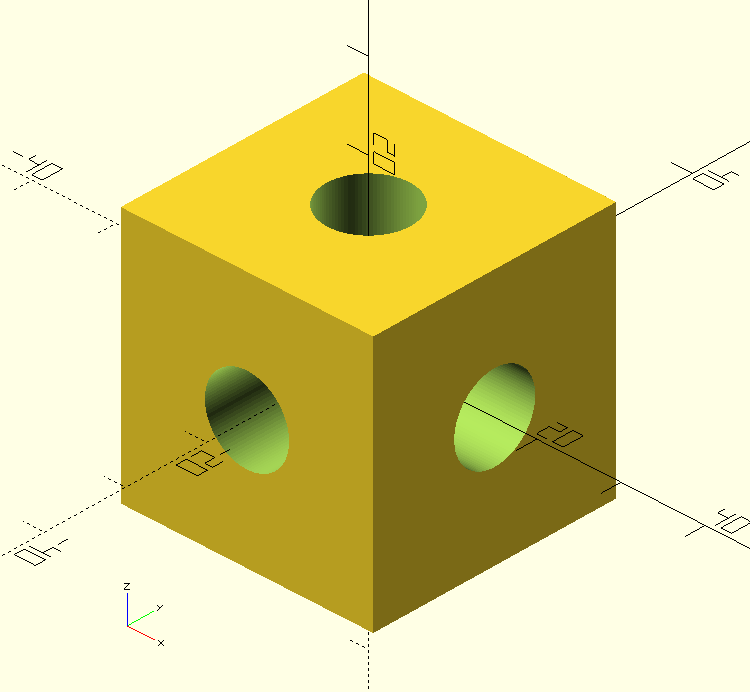
\includegraphics[width=.5\textwidth]{imagenes/diferencia-cubo-cilindros}      
      \caption{Tres cilindros perpendiculares restados a un cubo.}
      \label{fig:diferencia-cubo-cilindros}
    \end{figure}


    ---A ver ---Cecilia se entusiasmó y tomó el teclado---; dejame a
    mí:

  % \begin{center}
  % \begin{minipage}[]{1\textwidth}
    \begin{lstlisting}
$fn=100;
difference() {
  cube([30,30,30],center=true);
  for(vector=[[0,0,0],[90,0,0],[0,90,0]])
   rotate(vector)
    cylinder(h=60,r=5,center=true);
}
    \end{lstlisting}%$
% \end{minipage}\hfill

    \begin{figure}[ht]
      \centering
      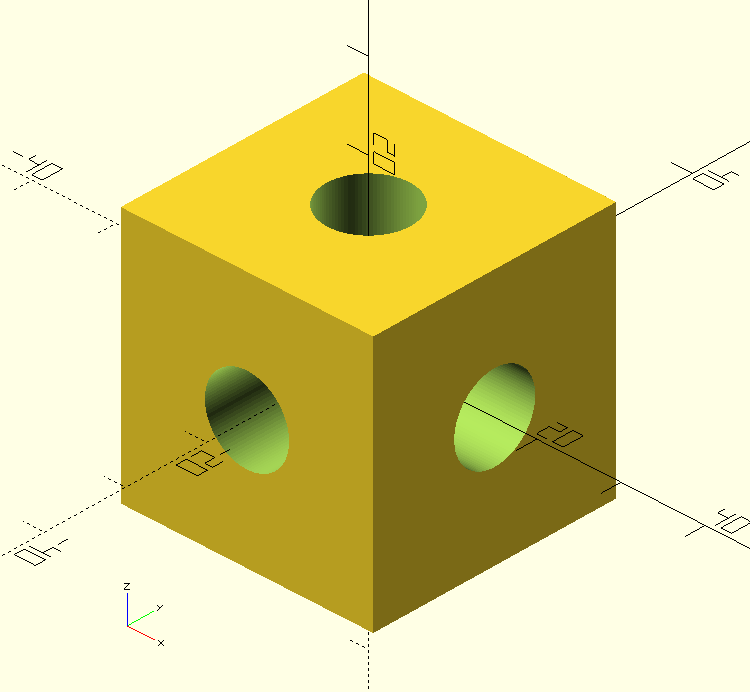
\includegraphics[width=.5\textwidth]{imagenes/diferencia-cubo-cilindros}      
      \caption{Tres cilindros perpendiculares restados a un cubo usando un bucle.}
      \label{fig:diferencia-cubo-cilindros-bucle}
    \end{figure}
    



---¡Cómo te gustaron los bucles! ---aprobó Antonia, y ambas rieron con ganas.

---Antonia ---Cecilia preguntó---, ¿era necesario que los cilindros
fueran más largos que el lado del cubo?

  Antonia frunció los labios:

  ---Pues, sí. En caso contrario, no resulta claro qué debería pasar
  con las `tapas': ¿deben permanecer (porque pertenecen al cuerpo
  inicial) o deben irse (porque pertenecen al cuerpo que se resta)? De
  hecho, fijate en la figura \ref{fig:diferencia-rara} lo que pasa si
  hago que los cilindros tengan la misma altura que el cubo:


  % \begin{center}
  % \begin{minipage}[]{1\textwidth}
    \begin{lstlisting}
$fn=100;
difference() {
  cube([30,30,30],center=true);
  for(eje=[[0,0,0],[90,0,0],[0,90,0]])
   rotate(eje)
    cylinder(h=30,r=5,center=true);
}
    \end{lstlisting}%$
% \end{minipage}\hfill

    
    \begin{figure}[ht]
      \centering
      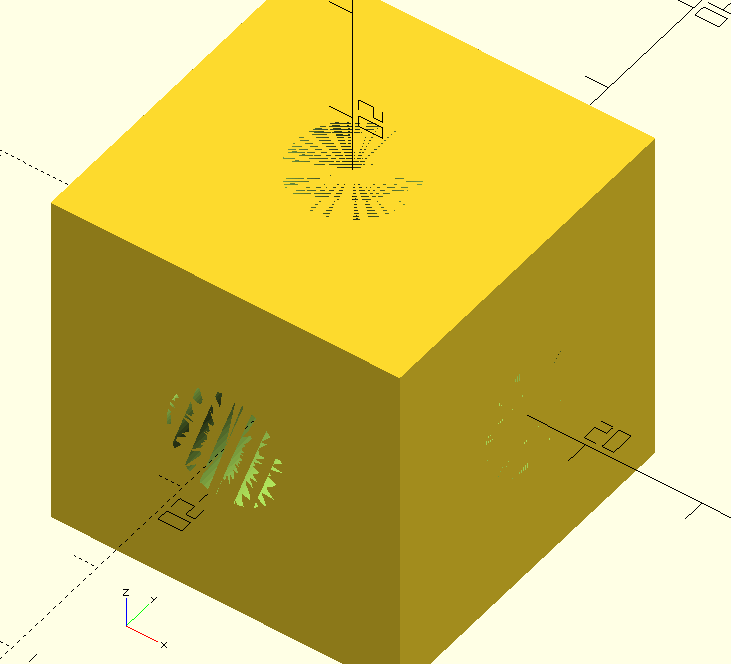
\includegraphics[width=.5\textwidth]{imagenes/diferencia-rara}      
      \caption{Los objetos sustraendo y minuendo no deben tener caras en común.}
      \label{fig:diferencia-rara}
    \end{figure}


    ---A propósito ---Antonia dedicó a Cecilia una mirada de
    ad\-mi\-ra\-ción---: gracias a tu reescritura del texto, sólo tuve
    que cambiar el `60' por el `30' una sola vez.

    Cecilia se sonrojó ligeramente, y salió del paso con rapidez:
    
    ---Ahí lo veo, es verdad: el propio \openscad{} pareciera indeciso
    acerca de qué hacer con esas `tapas'.

    ---Por esa razón conviene evitar toda ambigüedad haciendo los
    cuerpos `sustraendos' más grandes que el cuerpo `minuendo'
    ---sen\-ten\-ció Antonia.

    ---¡La última! ---Cecilia levantó bien alta la mano con una
    son\-ri\-sa---: ¿Por qué se escriben un par de paréntesis después de
    la palabra \lstinline!difference!?

    ---Ni idea ---fue la sincera y lacónica respuesta de Antonia.

  \section{Modificadores}


  ---¡Qué lastima que los cuerpos sustraendos desaparezcan!  Quiero
  decir ---Cecilia se explicó---, entiendo que si quiero restarlos, no
  deben permanecer; es obvio. Es sólo que siento que estoy escribiendo
  `a ciegas': me gustaría poder ver de alguna manera los objetos que
  estoy restando.

  ---Hay una solución a esa razonable inquietud ---re\-co\-no\-ció
  Antonia---: todo cuerpo precedido por el símbolo `\lstinline!#!' es
  dibujado en un tono rosado y transparente, sin importar si es
  sustraendo o no.



    \begin{lstlisting}
$fn=100;
difference() {
  cube([30,30,30],center=true);
  for(eje=[[0,0,0],[90,0,0],[0,90,0]])
    #rotate(eje)
      cylinder(h=30,r=5,center=true);
}
    \end{lstlisting}%$

    \begin{figure}[ht]
      \centering
      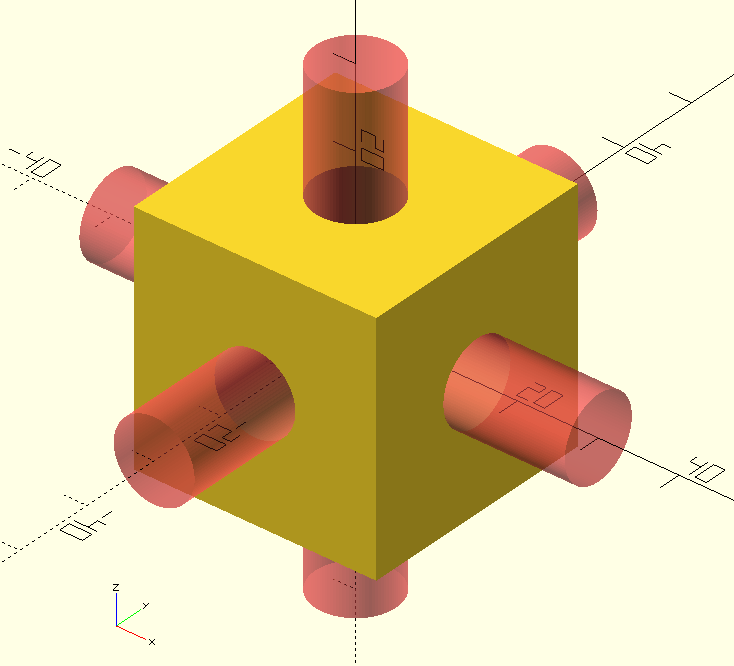
\includegraphics[width=.5\textwidth]{imagenes/diferencia-con-rosa}      
      \caption{Antonia emplea el modificador visual "\texttt{\#}".}
      \label{fig:diferencia-con-rosa}
    \end{figure}


    ---¡Hermoso! ---exclamó Cecilia, contemplando la figura
    \ref{fig:diferencia-con-rosa}.

    ---Hay más modificadores ---Antonia no ocultaba su regocijo cada
    vez que lograba despertar el entusiasmo en otra
    per\-so\-\mbox{na---.} Uno que me resulta muy útil,
    particularmente cuando trabajo con un texto con muchos objetos, es
    `\lstinline!!!': cuando precedés un objeto con él, \openscad{}
    ignora todos los demás y lo dibuja a él solo. Te permite así
    concentrarte en un objeto en particular, sin distraerte con los
    demás ---a\-cla\-ró y, tras unos instantes en los que pareció
    dudar, agregó---: A ver si lo encuentro...

Antonia estuvo un buen rato buscando en el desordenado árbol de
directorios de su computadora hasta que dio finalmente con el par de
imágenes de la figura \ref{fig:montura}.



  \begin{figure}[ht]
    \centering
    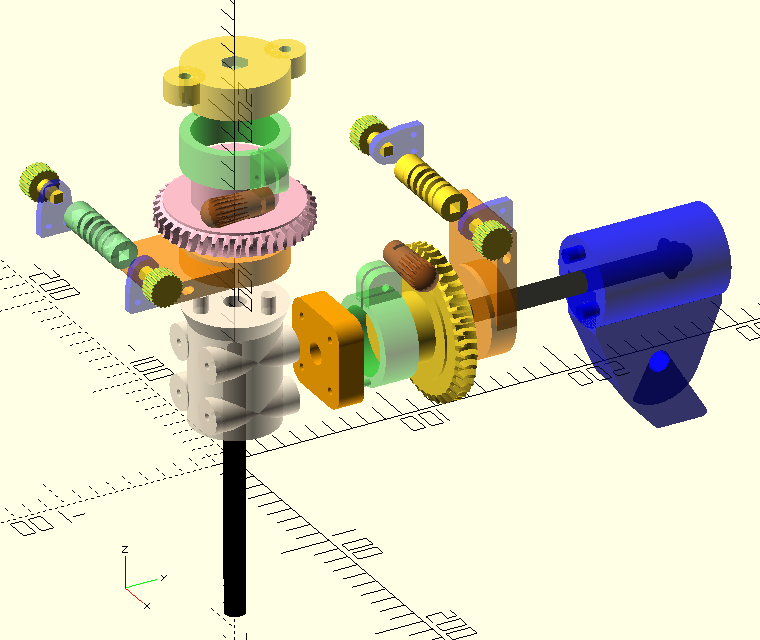
\includegraphics[width=.49\textwidth]{imagenes/montura-1}\hfill
    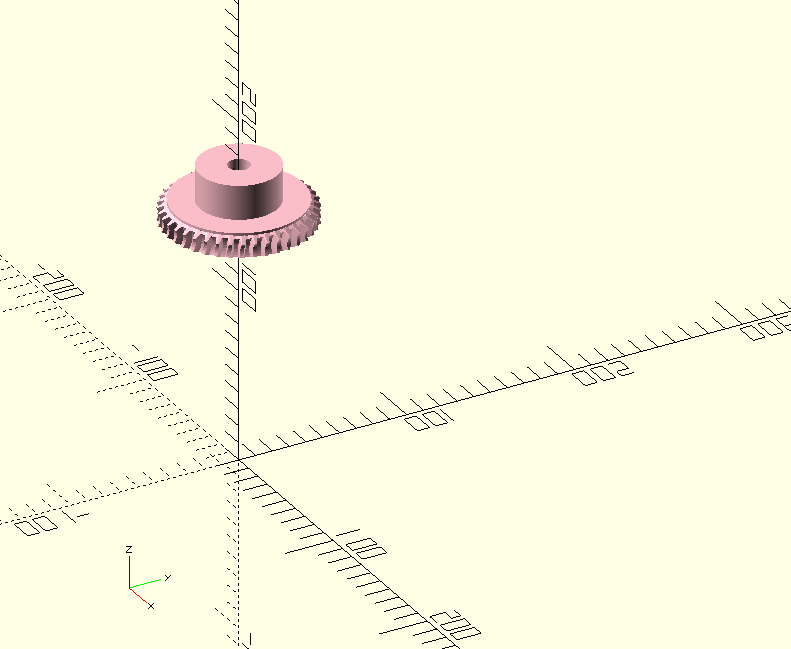
\includegraphics[width=.49\textwidth]{imagenes/montura-2}    
    \caption{Una montura ecuatorial alemana. Gracias al modificador
      ``\texttt{!}'', a la derecha sólo se muestra la corona del eje
      de declinación.}
    \label{fig:montura}
  \end{figure}




  Cecilia casi saltó de su silla:

  ---¿¡Y eso qué es!?  ---preguntó en lo que fácilmente podía
  confundirse con un grito.

  ---Nada ---respondió Antonia con gesto cansado---; una montura para
  un telescopio en la que vengo trabajando hace un tiempo con la
  esperanza de imprimirla algún día.\footnote{Asombrosamente, dicha
    montura no sólo fue terminada e impresa, sino incluso adosada a un
    telescopio actualmente en uso en el Observatorio donde desempeña
    sus tareas el autor. Debemos admitir también, no sin perplejidad,
    que hasta el momento no ha sido posible romperla ni malograrla;
    pero no dudamos de la labor eficaz del tiempo.}

  
  \section{El semicilindro (ahora sí)}

  ---Volvamos al semicilindro ---invitó Antonia---.  Creo que lo
  podemos resolver restando un cubo a un cilindro. Las dimensiones del
  cilindro `base' deben ser las mismas que las del semicilindro deseado
  por el usuario, e indicadas por los parámetros \texttt{h} y
  \texttt{r}. Sólo hay que tener cuidado de que el cubo sustraendo sea
  más grande, y esté debidamente trasladado; a ver...


    \begin{lstlisting}
module semicilindro(h,r){
  difference(){
    cylinder(h=h,r=r);
     #translate([-2*r,0,-h])
       cube([4*r,2*r,3*h]);
  }
}
semicilindro(40,5);
    \end{lstlisting}

    \begin{figure}[ht]
      \centering
      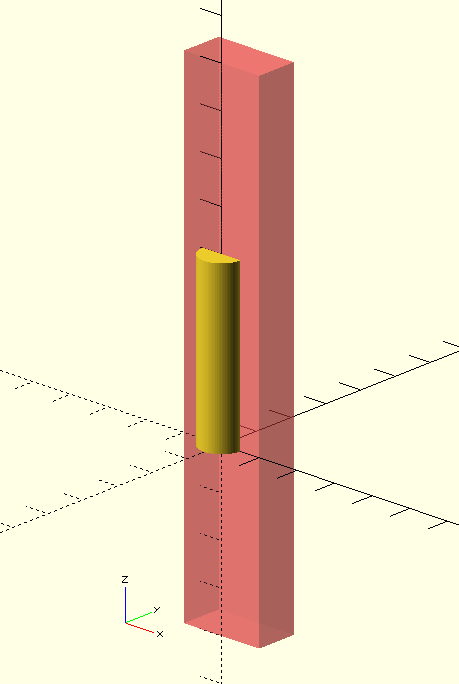
\includegraphics[width=.35\textwidth]{imagenes/semicilindro-1}      
      \caption{Módulo \texttt{semicilindro} en elaboración.}
      \label{fig:semicilindro-1}
    \end{figure}


    \guillemotright Para ir viendo cómo queda, y hasta que quedemos
    conformes con la definición final, yo diría que usemos el
    modificador `\lstinline!#!' para el cubo ---propuso Antonia.

    ---¡Eh! ---objetó Cecilia---. ¿No es demasiado grande el cubo?

    ---¿`Demasiado' para qué? ---se defendió Antonia---. Ese cubo no
    ocupa más lugar en la memoria de la computadora que uno
    visualmente más pequeño, y nos permite mantener el texto con
    números más manejables y discretos que 1,75, 2,5, u otros por el
    estilo.

    Cecilia, tras considerarlo unos instantes, sintió que su amiga
    tenía razón. En todo caso, tampoco parecía digno de discusión.

  Antonia recorría el texto con una mirada que trasuntaba una evidente
  insatisfacción:

  ---Hay algo que podemos mejorar ---lanzó finalmente---. Como sin
  duda recordarás, los cilindros admiten, al momento de ser creados,
  la indicación \lstinline!center=true!; considero que, a fin de
  cumplir con el `Principio de mínima perplejidad' \footnote{¡Ah!
    ¿Vieron? Antonia conocía ese principio, después de todo. (Nota del
    Editor)}, los semicilindros deberían también hacerlo:

  % \begin{center}
  % \begin{minipage}[]{1\textwidth}
    \begin{lstlisting}
module semicilindro(h,r,center=false){
  difference(){
    cylinder(h=h,r=r,center=center);
     #translate([-2*r,0,-h])
       cube([4*r,2*r,3*h]);
  }
}

semicilindro(40,5);

translate([100,0,0])
  semicilindro(40,5,center=true);
    \end{lstlisting}
  % \end{minipage}\hfill

    
    \begin{figure}[ht]
      \centering
      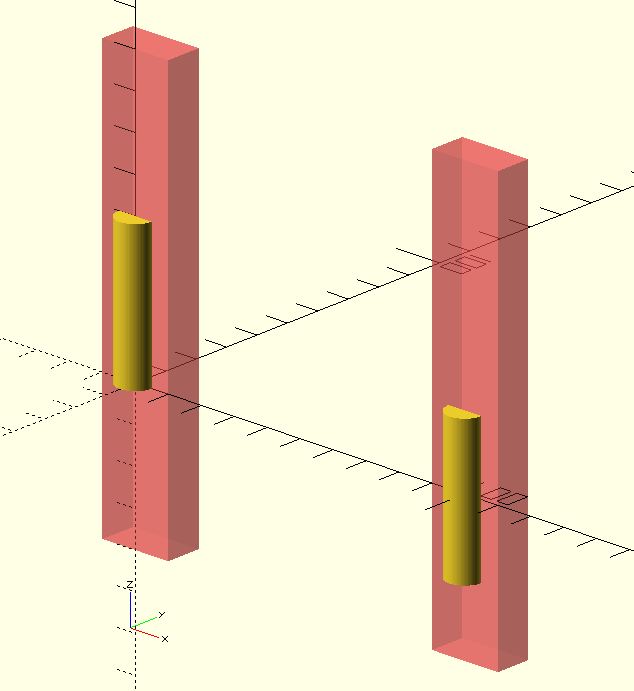
\includegraphics[width=.5\textwidth]{imagenes/semicilindros-center}      
      \caption{El módulo \texttt{semicilindro} acepta el parámetro \texttt{center}.}
      \label{fig:semicilindro-center}
    \end{figure}



    Cecilia tuvo que repasar mentalmente sus recuerdos de los
    parámetros opcionales. En principio, entendió que el semicilindro
    aceptaba un parámetro \lstinline!center!, con un valor
    preestablecido (o ``por defecto'', como les gusta traducir a
    algunos informáticos\footnote{Y hacen bien: la vigesimotercera
      edición del diccionario de la Real Academia admite la locución
      adverbial ``\emph{por defecto}'' en el sentido en que se emplea
      comúnmente en Informática y Tecnología.  (Nota del Editor)})
    igual a \lstinline!false!; es decir que, si el usuario no lo
    menciona (como ocurría en la línea 9 del nuevo texto), adoptaba
    ese valor. En caso contrario (como en la línea 12), puede tomar el
    valor \lstinline!true!. En cualquiera de ambos casos, el módulo
    \lstinline!semicilindro! pasa ese valor al parámetro
    \lstinline!center! del \lstinline!cylinder!: o sea, si el usuario
    escribe ``\lstinline!center=true!'', el \lstinline!cylinder! se
    crea con \lstinline!center=true!; en caso contrario, con
    \lstinline!center=false!. A Cecilia le pareció una solución muy
    limpita: un ``pase de manos'', por así decir. El trabajo de
    centrar el semicilindro resultaba finalmente responsabilidad del
    cilindro base, del cual podemos confiar que sabe muy bien cómo
    centrarse solo.

\section{Colores}
  
---Yo creo que la definición quedó bastante bien ---pro\-pu\-so Antonia,
guiñando un ojo---. ¡Vamos sacar el modificador `\lstinline!#!' y a
usar un poco nuestros semicilindros!

% \begin{center}
%   \begin{minipage}[]{1\textwidth}
\begin{lstlisting}
module barra_de_chocolate(){
 for (x=[0:10:100])
  translate([x,0,0])
   rotate([-90,0,0])
    semicilindro(h=50,r=5);
}
  
color("SaddleBrown")  
 barra_de_chocolate();
\end{lstlisting}
%  \end{minipage}\hfill


\begin{figure}[ht]
  \centering
  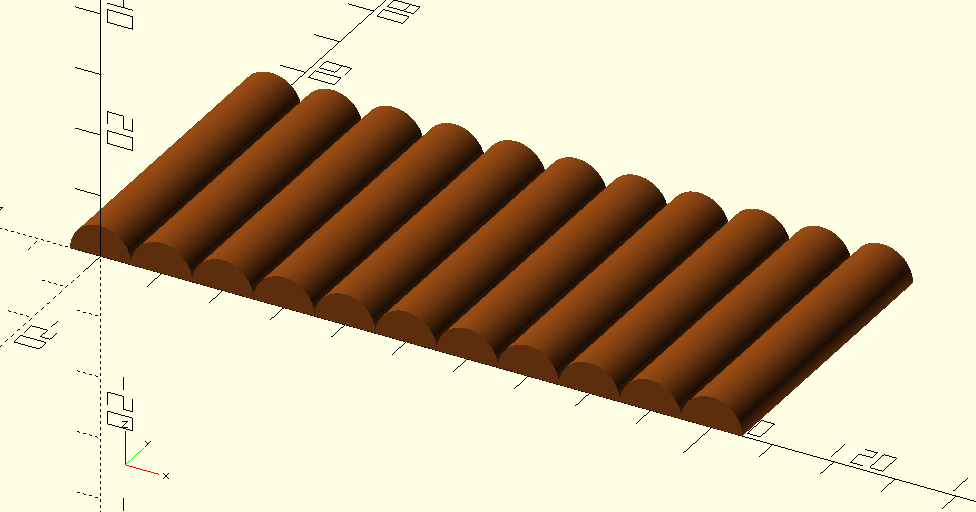
\includegraphics[width=.65\textwidth]{imagenes/barra-de-chocolate}  
  \caption{Una barra de chocolate... o algo así.}
  \label{fig:barra-de-chocolate}
\end{figure}

  
---Muy graciosa ---soltó Cecilia, que no siempre compartía el sentido
del humor de Antonia---. ¿Qué es eso de \lstinline!color!?

---Es una transformación más, como \lstinline!rotate! y
\lstinline!translate!; sólo que afecta meramente al color de la
visualización ---An\-to\-nia sonreía, divertida---. Puede usarse con el
nombre del color (de acuerdo a una prolija lista que puede consultarse
en
\url{https://en.wikibooks.org/wiki/OpenSCAD_User_Manual/Transformations\#color}),
o usando el clásico sistema de código RGB. Es posible, además, indicar
un factor de transparencia... en fin, los detalles te sugiero
consultarlos en la página cuya dirección acabo de copiarte.

Cecilia comprendió que Antonia no estuviera demasiado ansiosa por dar
más detalles: ya iban por la página
\pagedifferenceplusone{semicilindro-1}{semicilindro-1-final} del
capítulo, que fue bastante intenso.
\label{semicilindro-1-final}

%%% Local Variables:
%%% mode: latex
%%% TeX-master: "../libro"
%%% End:
